
\chapter{Labs with CVA6 Project}
\label{chapter:labs_with_cva6}


\begin{figure}[t]
    \centering
    \frame{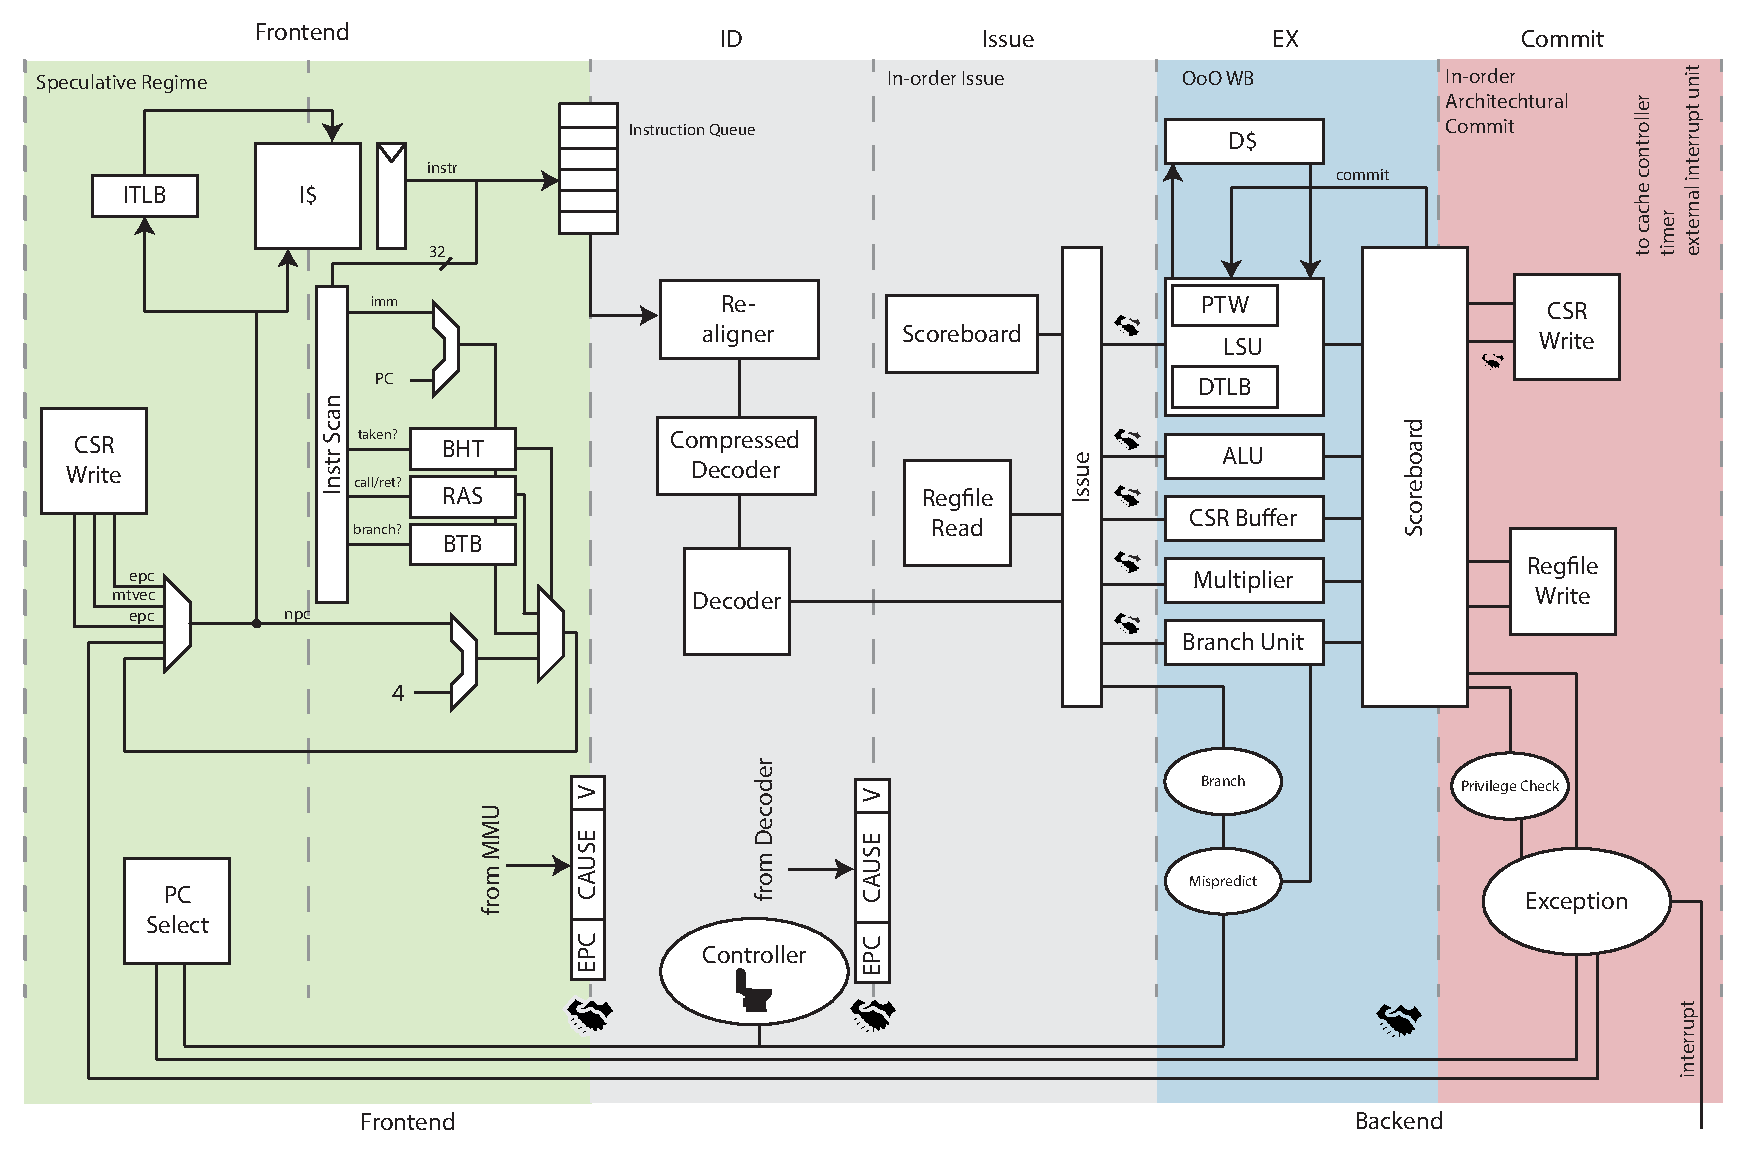
\includegraphics[width=0.7\linewidth]{media/cva6_overview.pdf}}
    \caption{CVA6 Block Diagram \cite{cva6}}
    \label{fig:cva6_overview}
\end{figure}


Standing as a culmination of all the Verilog education philosophies described in this thesis is a set of assignments I designed under the project label ``Labs with CVA6''. By drawing on my experiences from my time at Intel, my contributions to open-source projects, and interactions with industry contacts, I wrote four labs that aimed to give students practical experience with advanced computer architecture concepts. Each lab is centered around the fully featured RISC-V core CVA6, which is perfect for advanced architecture education due to its 6-stage pipeline, dynamic branch predictor, L1 cache, scoreboard unit, and virtual memory support (\autoref{fig:cva6_overview}). The labs presented students with a unique chance to engage with a fully-featured and transparent RISC-V core. This hands-on interaction facilitated a deeper comprehension of important architectural principles while also enhancing their ability to work with large and complex SystemVerilog designs. These labs are available for free under the BSD-3-Clause license \cite{labsWithCVA6}.

\section{These labs provide hands-on exploration of architectural concepts.}

For instance, the Branch Prediction Lab guided students in modifying CVA6 simulations to display hit rate results and in adapting the CVA6 branch prediction unit into a global predictor. [fig] Similarly, the Caching Lab showed students how to incorporate a victim-cache module, then required creation of an assembly script to demonstrate an understanding of how the cache hierarchies and memory management would be affected. [fig] Then moving away from custom RTL, in the Out-of-Order Lab, students further practiced writing assembly programs to test their comprehension of out-of-order execution by demonstrating data hazards. [fig] Finally, the Virtual Memory Lab enabled students to configure privilege modes and set up page-table entries by modifying an assembly program that acted as a simple bootloader and OS. [fig] Each of these labs were only made possible with CVA6's open-source framework. Based on ECE 154B student responses and post-lab discussions, it was evident that the practical insights offered by these labs substantially deepen understanding of the concepts.

\section{There is high demand for hands-on learning experiences.}

Because ``Labs with CVA6'' is available under the BSD-3-Clause license, it has attracted attention from many non-ECE 154B audiences including instructors seeking to enrich their own architecture courses, researchers aiming to familiarize themselves with the specifics of CVA6, and SystemVerilog beginners eager to learn best-practices. In addition, I gave a well-appreciated talk about ``Labs with CVA6'' at ``Latch-Up'', a conference hosted by The Free and Open Source Silicon Foundation \cite{SiffermanLatchUp}. During my presentation, I expressed the practical and unique skills that students acquire through studying the code of well-verified, open-source designs. This resonated deeply with several attendees, especially Rick O'Connor, the President and CEO at OpenHW Group, who notified me of the new RISC-V core, CV-Wally \cite{cvwally}, that is designed as a supplemental codebase for the upcoming textbook, ``RISC-V System-on-Chip Design''. The popularity that ``Labs with CVA6'' has seen, and the recent creation of CV-Wally shows that there is strong demand for curriculums that offer transparency on implementation methods of real-world designs.
